\subsection{Pattern selectors}
\label{sub:learning:selectors}

% ----------------------- paths to graphics ------------------------

\graphicspath{{5_automatic_learning/learning_process/images/}}

% ----------------------- contents from here ------------------------
% 

Section \ref{sub:learning:recursiveexhaustive} described an exhaustive learning algorithm based on compression estimators (\ref{sub:estimators}). A greedy learning algorithm based on \emph{pattern selectors} will be described in section \ref{sub:learning:iterative}. Pattern selectors are decision algorithms used to make greedy choices in the compression learning process. This section describes the general characteristics of a pattern selector and specialized instances of it.

\subsubsection{Generic pattern selector}
\label{subsubsec:ps:generic}

A generic pattern selector is an abstraction used in the learning process for selecting the \textit{expression nodes} that will be added to the compression tree. Given a list of \textit{(expression node, evaluation result)} tuples resulted in the pattern detection phase, it outputs a subset of the expression trees provided as input. This selection process is necessary as there are multiple ways of representing the same column. The generic pattern selector chooses the best \textit{expression nodes} according to a set of criteria. Different implementations of pattern selectors are described below.

TODO-2: [?] image describing the input and output of the generic pattern selector; not necessary but may be added for completeness and for reuse in the learning algorithms diagrams

\subsubsection{Coverage pattern selector}
\label{subsubsec:ps:coverage}

The coverage pattern selector tries to maximize the coverage of each column (i.e. minimize the exception ratio). It has 2 operation modes: 1) \textit{single-pattern}: selects the \textit{expression node} with the highest coverage; 2) \textit{multi-pattern}: selects the best combination of \textit{expression nodes} that give the largest coverage when used together on the same column.

The values on a column usually fall in different, possibly overlapping, pattern types. It is rarely the case that one pattern perfectly fits to all the values in a column. In most cases there is either one dominant pattern and the rest of the values are just noise, or multiple patterns that together cover all the values on the column. An example could be a \verb|VARCHAR| column where half of the values are numbers and the other half are concatenations of a constant with numbers.

The \textit{single-pattern} operation mode will select only one expression node---the one with the highest coverage. The \textit{multi-pattern} operation mode will select multiple expression nodes, such that their combined coverage of the column is maximal. We defined 2 approaches for the \textit{multi-pattern} mode: 1) a Greedy algorithm that selects one expression node at a time---the one with the highest coverage---until the column is fully covered or there are no more expression nodes to choose from; 2) an exhaustive algorithm that tries every combination of expression nodes and outputs the one with the highest cumulative coverage. Both approaches can further take into account the following parameter: \(coverage_{min}\)---minimum coverage that determines whether a pattern is considered or not.

The combined coverage of 2 patterns \(p_{a}\) and \(p_{b}\) can be computed based on their \textit{row\_masks} \(\mathit{rm}_{a}\), \(\mathit{rm}_{b}\)---defined in \ref{subsec:genericpd}---through a bitwise \verb|OR| operation: \(\mathit{rm}_{combined} = \mathit{rm}_{a} | \mathit{rm}_{b}\). The number of bits of a \textit{row\_mask} is equal to the number of rows in the table: \(r\). The combined coverage is then computed as the number of \(1\) bits in \(\mathit{rm}_{combined}\) divided by \(r\).

The complexity of these algorithms depends on the number of patterns found on the column: \(p\). The \textit{single-pattern} operation mode and the Greedy algorithm for the \textit{multi-pattern} mode both have a linear complexity. The exhaustive algorithm has an exponential complexity, as it tries all combinations of patterns: for \(p = 10\) there are \(10^3\) bitwise \verb|OR| operations on \(r\)-bit numbers, while for \(p = 27\) this number grows to \(10^9\). Equation~\ref{eq:ps:coverage:exhaustive} shows the complexity of the exhaustive algorithm.
\begin{equation}
\label{eq:ps:coverage:exhaustive}
    \sum_{k=1}^{p} {p \choose k}
\end{equation}

We implemented a basic version of the exhaustive approach for the \textit{multi-pattern} mode. To avoid the exponential running time, we default to the \textit{single-pattern} mode if the number of patterns \(p\) is larger than 20. In practice, we never encountered more than 20 different patterns on the same column, therefore, the exhaustive approach is a suitable choice.

Both operation modes give similar results in terms of physical representation of the data, but the resulting expression trees have different shapes. The \textit{single-pattern} mode selects only one expression node, moving the other values on an exception column. If the learning algorithm supports recursive expression of exception columns, then the most dominant pattern in the exception column is further selected, resulting in a new expression node on a new level of the tree. This process creates deep expression trees. In contrast, the \textit{multi-pattern} mode adds all expression nodes on the same level of the tree, resulting in wider but shorter expression trees. The evaluation of expression trees resulted from \textit{multi-pattern} selection is described in \ref{sec:exprlang:compdecomp}~\nameref{sec:exprlang:compdecomp}.

TODO-1: images with the 2 types of compression trees (deep and wide)

\subsubsection{Priority pattern selector}
\label{subsubsec:ps:priority}

The purpose of this pattern selector is to choose the best expression node based on pattern priorities. In addition to the \textit{expression node} list, it also receives a set of priority classes for pattern detector types. Each priority class contains a list of pattern types (e.g. \nameref{subsec:pd:numericstrings}, \nameref{subsec:pd:charsetsplit}, etc.) and a pattern selector that will be used to select the patterns in the same class. The selection process works in the following way:\\
1) for each column, select only the \textit{expression nodes} with the highest priority---their associated pattern type has the highest priority according to the provided list\\
2) further select these \textit{expression nodes} using the pattern selector provided for their priority class and output the result

An example of an input priority set is shown in Table~\ref{tab:ps:priority:table1}.

\begin{table}[h]
\centering
\begin{tabular}{@{}cll@{}}
\toprule
\multicolumn{1}{l}{Priority} & Pattern type               & Pattern selector  \\ \midrule
1                            & Constant                   & N/A               \\
2                            & Dictionary, Numeric string & Coverage selector \\
3                            & Character set split        & Coverage selector \\ \bottomrule
\end{tabular}
\caption{Priority set example}
\label{tab:ps:priority:table1}
\end{table}


Given a column \(c\) and the priority set in Table~\ref{tab:ps:priority:table1}, the \nameref{subsubsec:ps:priority} will proceed as follows. It will first search for a \nameref{subsec:pd:constant} expression node that has \(c\) as input. If found, \(c\) will be represented as a constant. Since the \nameref{subsec:pd:constant} pattern detector outputs only one result per column, there is no need for a pattern selector on the constant priority class---the only constant expression node will be chosen. If there is no constant expression node, the pattern selector will search for expression nodes in the next priority class: \nameref{subsec:pd:dict} and \nameref{subsec:pd:numericstrings}. Both pattern detectors output a single result per column, thus there is a maximum of 2 expression nodes to choose from. The \nameref{subsubsec:ps:coverage} will be used to choose between them. Finally, if no expression node was found yet, the selector moves to the last priority class. It searches for \nameref{subsec:pd:charsetsplit} expression nodes.
There can be multiple instances of the \nameref{subsec:pd:charsetsplit} pattern detector initialized with different parameters and each instance can output multiple results for the same column. The \nameref{subsubsec:ps:coverage} is used to choose the best combination of results such that the total coverage of the column is maximized.

\subsubsection{Correlation pattern selector}
\label{subsubsec:ps:correlation}

This pattern selector is specialized in \nameref{subsec:pd:columncorrelation} \textit{expression nodes}. The \nameref{subsec:pd:columncorrelation} pattern detector outputs all the correlations between the columns in the dataset, resulting in multiple possibilities of representing the same column as a function of other columns---multiple \textit{(source, target)} pairs with the same target column. The \nameref{subsubsec:ps:correlation} selects the \textit{expression nodes} such that every \textit{target} column is represented by a single \textit{source} column, while also trying to maximize the average correlation coefficient and avoid circular dependencies.

We can make the following observation: the column correlation as defined in \ref{subsec:pd:columncorrelation} is a transitive relation. We formalized this observation in Theorem~\ref{subsec:ps:corr:theorem1}.

\begin{theorem}
\label{subsec:ps:corr:theorem1}
Let \(c_{a}\), \(c_{b}\), \(c_{c}\) be three columns and let \(c_{a} \xrightarrow{m_{ab}} c_{b}\) be the correlation relation meaning: \(c_{a}\) determines \(c_{b}\) through a mapping \(m_{ab}\). If \(c_{a} \xrightarrow{m_{ab}} c_{b}\) and \(c_{b} \xrightarrow{m_{bc}} c_{c}\) then \(c_{a} \xrightarrow{m_{ac}} c_{c}\).
\end{theorem}
\begin{proof}
Let \((v_{a}, v_{b})\) be an entry in \(m_{ab}\)---meaning: value \(v_{a}\) on column \(c_{a}\) always corresponds to value \(v_{b}\) on column \(c_{b}\)---and let \((v_{b}, v_{c})\) be an entry in \(m_{bc}\). Then, value \(v_{a}\) on column \(c_{a}\) always corresponds to value \(v_{c}\) on column \(c_{c}\). Therefore, \(\exists\) \(m_{ac}\)---a mapping containing the entry \((v_{a}, v_{c})\)---and \(c_{a} \xrightarrow{m_{ac}} c_{c}\).
\end{proof}

We define the correlation graph as follows: directed graph with one or more connected components; nodes represent columns; \textit{(src, dst)} edges represent correlations: column \textit{dst} is determined by column \textit{src}. The weight of an edge is the correlation coefficient between \textit{src} and \textit{dst}. An example of a correlation graph is shown in Figure~\ref{fig:ps:columncorrelation:corrgraph1}. The red edges represent an optimal selection in terms of the metrics and conditions described in the following paragraphs. This figure shows a simple correlation graph, but in practice we encountered much complex graphs resulted from the learning process for tables with highly correlated data.

\begin{figure}[h]
  \centering
  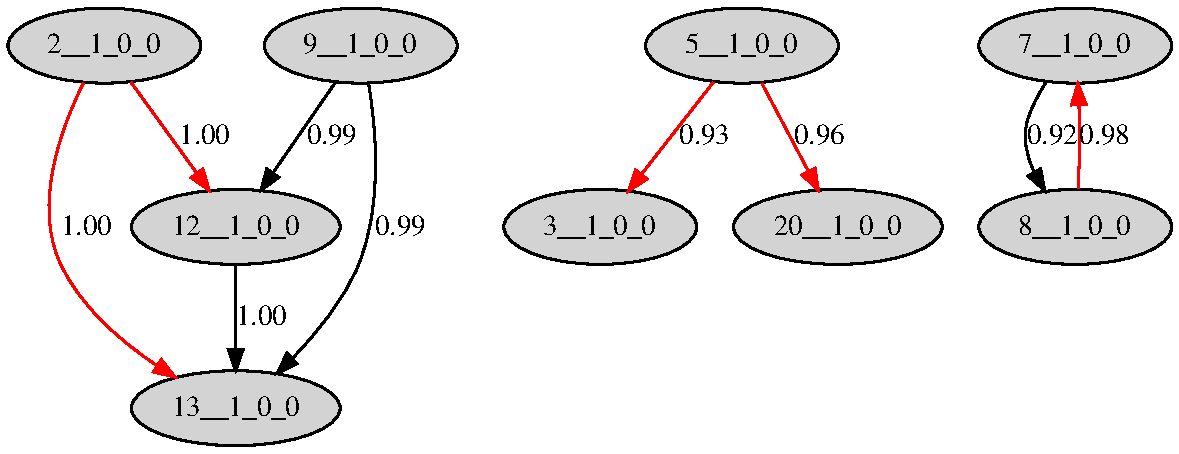
\includegraphics[width={0.9\linewidth}]{corr_graph_1.pdf}
  \caption{Correlation graph}
  \label{fig:ps:columncorrelation:corrgraph1}
\end{figure}

The main goal of the \nameref{subsubsec:ps:correlation} is to select a subset of the edges in the graph. We can define this process as the optimization problem of selecting a subset of edges in the correlation graph \(G\) such that the resulting subgraph \(G_{s}\) satisfies the following properties (in this order):
\begin{itemize}
    \item[\textit{P1}:] the indegree of any node is at most 1---a column should be determined by no more than 1 other column
    \item[\textit{P2:}] any path in \(G_{s}\) is of length 1---because of the transitivity property, for every path between nodes \(c_{a}\) and \(c_{b}\), there will also be a direct edge from \(c_{a}\) to \(c_{b}\)
    \item[\textit{P3}:] the number of nodes in \(G_{s}\) with indegree > 0 is maximal---the number of columns that are represented as functions of other columns is maximal
    \item[\textit{P4}:] the average weight of the edges is maximal---the edges with the highest correlation coefficient should be selected
\end{itemize}

We defined a Greedy algorithm for solving the correlation selection optimization problem. It builds the \(G_{s}\) graph by greedily selecting one edge at a time from \(G\). The edge is added to \(G_{s}\), \(G\) is updated and the process goes on until there are no more edges in \(G\). The algorithm is described in listings \ref{lst:ps:corr:selectcorr}, \ref{lst:ps:corr:nodescore}, \ref{lst:ps:corr:edgescore}.

\begin{lstlisting}[language=Python,
label={lst:ps:corr:selectcorr},
caption={select\_correlations}]
# G = correlation graph resulted from the correlation detection process
def select_correlations(G):
  G_s = <empty correlation graph>
  while G.edges is not empty:
    # select destination node
    dst = min(G.nodes, key=get_node_score)
    # select (_, dst) edge
    (src, dst, corr_coef) = min(dst.incoming_edges, key=get_edge_score)
    # update G_s
    G_s.add((src, dst, corr_coef))
    # update G
    G.remove(dst.incoming_edges)
    G.remove(dst.outgoing_edges)
    G.remove(dst)
    G.remove(src.incoming_edges)
  return G_s
\end{lstlisting}

\begin{lstlisting}[language=Python,
label={lst:ps:corr:nodescore},
caption={get\_node\_score}]
def get_node_score(node):
  indegree_src = min([src.indegree 
                     for (src, dst) in node.incoming_edges])
  return (node.outdegree, indegree_src, node.indegree)
\end{lstlisting}

\begin{lstlisting}[language=Python,
label={lst:ps:corr:edgescore},
caption={get\_edge\_score}]
def get_edge_score((src, dst, corr_coef)):
  return (src.indegree, -corr_coef, -src.out_degree)
\end{lstlisting}
\bigskip

Every iteration of the \textit{while} loop first selects the destination node of the candidate edge based on its score. The \textit{get\_node\_score} function prioritizes nodes with the minimum outdegree---ideally 0---such that the number of discarded edges as an effect of constraint \textit{P2} is minimized. The difference between nodes with the same outdegree is made by the minimum indegree of its parent nodes (source nodes of incoming edges)---for the same reason. Finally the difference is further made by the smallest indegree of the node itself, prioritizing columns with fewer options of being represented as functions of other columns. 

With the destination node fixed, the best edge is selected from its incoming edges. The \textit{get\_edge\_score} function prioritizes edges that have a minimum indegree---ideally 0---such that nodes at the start of correlation paths are selected. The difference between these nodes is further made based on the highest correlation coefficient and then by the highest outdegree.

The selected edge is added to \(G_{s}\) and \(G\) is updated such that constraints \textit{P1} and \textit{P2} are satisfied: the destination node, its incoming and outgoing edges and the incoming edges of the source node are removed. This process changes the degree of the nodes in \(G\) and impacts their scores.

The complexity of the algorithm, as described above, is given by the number of nodes in \(G\) and their average indegree: \(N^2 \times avg(indegree)\), where \(N\) is the number of nodes. Every iteration of the \textit{while} loop selects one node from \(G\) by computing the score of all nodes. The \textit{get\_node\_score} function loops through all incoming edges of the node. If the selection of the \(dst\) node is done with a priority queue the complexity is improved: \(N \times \log(N) \times avg(indegree)\).

An alternative approach would be to relax constraint \textit{P2} and allow paths of length higher than 1. Then apply a variation of the Dijkstra's shortest paths algorithm to shorten these paths with the goal of minimizing the complexity of the graph without affecting its average correlation coefficient. However, relaxing  \textit{P2} imposes a new constraint on \(G_{s}\): it should not contain any cycles. We leave this approach for future work.

% ---------------------------------------------------------------------------
% ----------------------- end of thesis sub-document ------------------------
% ---------------------------------------------------------------------------